\iffalse
% #######################################
% ########### FILL THESE IN #############
% #######################################
\def\mytitle{MATRICES}
\def\mykeywords{}
\def\myauthor{GOWTHAMI MANDAVA}
\def\contact{gowthamimandava999@gmail.com}
\def\mymodule{ Future Wireless Communication(FWC22012)}
% #######################################
% #### YOU DON'T NEED TO TOUCH BELOW ####
% #######################################
\newcommand{\myvec}[1]{\ensuremath{\begin{pmatrix}#1\end{pmatrix}}}
\let\vec\mathbf
\providecommand{\pr}[1]{\ensuremath{\Pr\left(#1\right)}}
\providecommand{\qfunc}[1]{\ensuremath{Q\left(#1\right)}}
\providecommand{\sbrak}[1]{\ensuremath{{}\left[#1\right]}}
\providecommand{\lsbrak}[1]{\ensuremath{{}\left[#1\right.}}
\providecommand{\rsbrak}[1]{\ensuremath{{}\left.#1\right]}}
\providecommand{\brak}[1]{\ensuremath{\left(#1\right)}}
\providecommand{\lbrak}[1]{\ensuremath{\left(#1\right.}}
\providecommand{\rbrak}[1]{\ensuremath{\left.#1\right)}}
\providecommand{\cbrak}[1]{\ensuremath{\left\{#1\right\}}}
\providecommand{\lcbrak}[1]{\ensuremath{\left\{#1\right.}}
\providecommand{\rcbrak}[1]{\ensuremath{\left.#1\right\}}}
\documentclass[10pt, a4paper]{article}
\usepackage[a4paper,outer=1.5cm,inner=1.5cm,top=1.75cm,bottom=1.5cm]{geometry}
\twocolumn
\usepackage{circuitikz}
\usepackage{amsmath,bm}
\usepackage{amsthm}
\usepackage{mathtools}
\usepackage{amsfonts}
\usepackage{amssymb}
\usepackage{graphicx}
\graphicspath{{./images/}}
%colour our links, remove weird boxes
\usepackage[colorlinks,linkcolor={black},citecolor={blue!80!black},urlcolor={blue!80!black}]{hyperref}
%Stop indentation on new paragraphs
\usepackage[parfill]{parskip}
%% Arial-like font
\usepackage{lmodern}
\renewcommand*\familydefault{\sfdefault}
%Napier logo top right
\usepackage{watermark}
%Lorem Ipusm dolor please don't leave any in you final report ;)
\usepackage{karnaugh-map} 
\usepackage{tabularx}
\usepackage{lipsum}
\usepackage{xcolor}
\usepackage{listings}
%give us the Capital H that we all know and love
\usepackage{float}
%tone down the line spacing after section titles
\usepackage{titlesec}
%Cool maths printing
\usepackage{amsmath}
%PseudoCode
\usepackage{algorithm2e}

\titlespacing{\subsection}{0pt}{\parskip}{-3pt}
\titlespacing{\subsubsection}{0pt}{\parskip}{-\parskip}
\titlespacing{\paragraph}{0pt}{\parskip}{\parskip}
\newcommand{\figuremacro}[5]{
    \begin{figure}[#1]
        \centering
        \includegraphics[width=#5\columnwidth]{#2}
        \caption[#3]{\textbf{#3}#4}
        \label{fig:#2}
    \end{figure}
}


 \lstset{
frame=single, 
breaklines=true,
columns=fullflexible
}

\thiswatermark{\centering \put(1,-110){\includegraphics[scale=0.05]{IIT_logo.jpg}} }
\title{\mytitle}
\author{\myauthor\hspace{1em}\\\contact\\IITH\hspace{0.5em}-\hspace{0.5em}\mymodule}
\date{}
\hypersetup{pdfauthor=\myauthor,pdftitle=\mytitle,pdfkeywords=\mykeywords}
\sloppy
% #######################################
% ########### START FROM HERE ###########
% #######################################
\begin{document}
 \maketitle
 \tableofcontents
 
    
 

 
    
    
    
 
 \Large\section{Problem}
 \fi
Find the equation of the line  parallel to the line 3x-4y+2=0 and passing through the point (-2,3).
\\
\solution 
\iffalse
 \section{Solution}
 \begin{center}
 Given equation is 3x-4y+2=0
\\the parallel line passing through point(-2,3)
\begin{align}
\textbf{n}^{\top}(\textbf{x}-\textbf{p})=0 
\end{align}
\label{tab:truthtable}
    \setlength{\arrayrulewidth}{0.2mm}
\setlength{\tabcolsep}{5pt}
\renewcommand{\arraystretch}{1.25}
    \begin{tabular}{|c|c|}
    \hline % <-- Alignments: 1st column left, 2nd middle and 3rd right, with vertical lines in between
      \large\textbf{Symbol} & \large\textbf{Co-ordinates} \\
      \hline
       \large \textbf{n} & $\ \begin{pmatrix} 3\\ -4 \end{pmatrix}$  \\
       \hline
       \large p & $\ \begin{pmatrix} -2\\ 3 \end{pmatrix}$ \\
       \hline
       	\large c & 2 \\
      \hline
   \end{tabular}
\\ by substituting we get
\fi
From the given information, 
\begin{align}
{\vec{n}}=\myvec{3\\-4} \\
\implies 
	\myvec{3&-4}\cbrak{\vec{x}-\myvec{-2\\3}}&=0
	\\
	&=-18 
\end{align}
which is the required equation of the line.
\iffalse
  therefore,the equation parallel to the given equation and passing through the point(-2,3) is 3x-4y+18=0
 \end{center}
 \section{Plot}
         \centering
        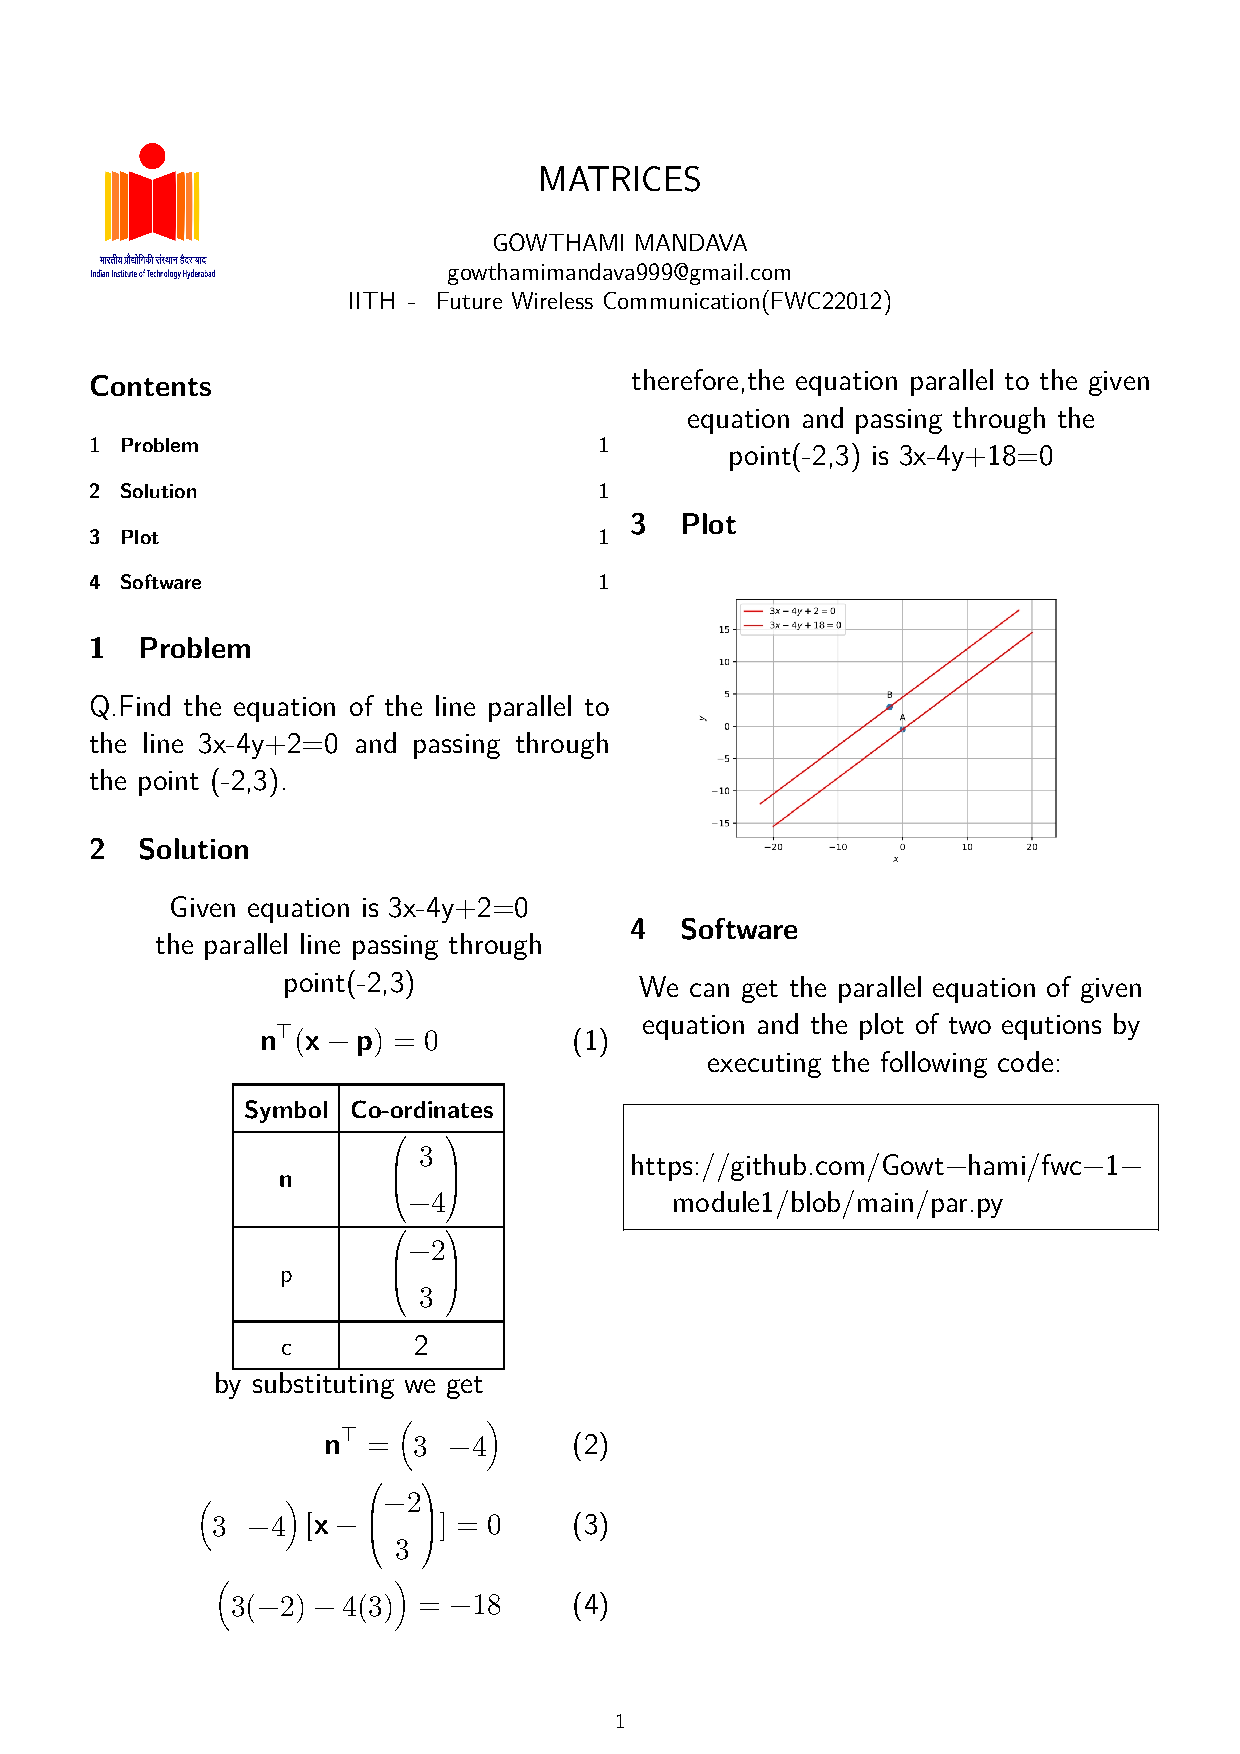
\includegraphics[scale=0.275]{mat.jpg}
  \section{Software}
  We can get the parallel equation of given equation and the plot of two equtions by executing the following code:
 \vspace{3mm} 
\begin{lstlisting}

https://github.com/Gowt-hami/fwc-1-module1/blob/main/par.py
\end{lstlisting}
\end{document}
\fi
